\documentclass[UTF8, 12pt]{ctexart}
% UTF8编码,ctexart现实中文
\usepackage{color}
% 使用颜色
\definecolor{orange}{RGB}{255,127,0} 
\definecolor{violet}{RGB}{192,0,255} 
\definecolor{aqua}{RGB}{0,255,255} 
\usepackage{geometry}
\setcounter{tocdepth}{4}
\setcounter{secnumdepth}{4}
% 设置四级目录与标题
\geometry{papersize={21cm,29.7cm}}
% 默认大小为A4
\geometry{left=3.18cm,right=3.18cm,top=2.54cm,bottom=2.54cm}
% 默认页边距为1英尺与1.25英尺
\usepackage{indentfirst}
\setlength{\parindent}{2.45em}
% 首行缩进2个中文字符
\usepackage{setspace}
\renewcommand{\baselinestretch}{1.5}
% 1.5倍行距
\usepackage{amssymb}
% 因为所以
\usepackage{amsmath}
% 数学公式
\usepackage[colorlinks,linkcolor=black,urlcolor=blue]{hyperref}
% 超链接
\usepackage{tikz}
% 绘图
\author{Didnelpsun}
\title{多元函数积分学}
\date{}
\begin{document}
\maketitle
\pagestyle{empty}
\thispagestyle{empty}
\tableofcontents
\thispagestyle{empty}
\newpage
\pagestyle{plain}
\setcounter{page}{1}
\section{二重积分}

\subsection{概念}

\subsubsection{几何背景}

二重积分的几何背景就是曲顶柱体的体积。定积分用极限的思想求出了二维平面的曲边梯形的面积,同样二重积分$\iint\limits_Df(x,y)\,\textrm{d}\sigma$。

被积函数$f(x,y)$作为曲顶柱体在点$(x,y)$处柱体微元的高,用底面积$\textrm{d}\sigma>0$乘上高$f(x,y)$就得到一个小柱体体积,再把所有$D$上的柱体相加起来就是整个曲顶柱体的体积。

\subsubsection{性质}

\begin{itemize}
    \item 求区域面积:$\iint\limits_D1\cdot\textrm{d}\sigma=\iint\limits_D\textrm{d}\sigma=A$,其中$A$为$D$的面积。
    \item 可积函数必有界:当$f(x,y)$在有界闭区间$D$上可积时,$f(x,y)$在$D$上必有界。
    \item 积分线性性质:$k_1,k_2$为常数,则$\iint\limits_D[k_1f(x,y)\pm k_2g(x,y)]\,\textrm{d}\sigma=\iint\limits_{D_1}f(x,y)\,\textrm{d}\sigma$\\$\pm k_2\iint\limits_{D_2}f(x,y)\,\textrm{d}\sigma$。
    \item 积分可加性:当$f(x,y)$在有界闭区间$D$上可积时,且$D_1\cup D_2=D$,$D_1\cap U_2=\varnothing$,则$\iint\limits_Df(x,y)\,\textrm{d}\sigma=\iint\limits_{D_1}f(x,y)\,\textrm{d}\sigma+\iint\limits_{D_2}f(x,y)\,\textrm{d}\sigma$。
    \item 积分保号性:当$f(x,y),g(x,y))$在有界闭区间$D$上可积时,若在$D$上有$f(x,y)\leqslant g(x,y)$,则$\iint\limits_Df(x,y)\,\textrm{d}\sigma\leqslant\iint\limits_Dg(x,y)\,\textrm{d}\sigma$,特别$\left\vert\iint\limits_Df(x,y)\,\textrm{d}\sigma\right\vert\leqslant\iint\limits_D\vert f(x,y)\vert\,\textrm{d}\sigma$。
    \item 二重积分估值定理:设$M,m$,分别为$f(x,y)$在有界闭区域$D$上的最大值和最小值,$A$为$D$的面积,则有$mA\leqslant\iint\limits_Df(x,y)\,\textrm{d}\sigma\leqslant MA$。
    \item 二重积分中值定理:设函数$f(x,y)$在有界闭区域$D$上连续,$A$为$D$的面积,则在$D$上至少存在一点$(\xi,\eta)$使得$\iint\limits_Df(x,y)\,\textrm{d}\sigma=f(\xi,\eta)A$。
\end{itemize}

\textbf{例题:}设$I_1=\iint\limits_D\cos\sqrt{x^2+y^2}\,\textrm{d}\sigma$,$I_2=\iint\limits_D\cos(x^2+y^2)\,\textrm{d}\sigma$,$I_3=\iint\limits_D\cos(x^2+y^2)^2\,\textrm{d}\sigma$,其中$D=\{(x,y)|x^2+y^2\leqslant1\}$,则()。

$A.I_3>I_2>I_1$\qquad$B.I_1>I_2>I_3$\qquad$C.I_2>I_1>I_3$\qquad$D.I_3>I_1>I_2$

解:令$x^2+y^2=t$,$\therefore0<t\leqslant1$。所以$1\geqslant\sqrt{t}\geqslant t\geqslant t^2\geqslant0$。

又$\cos x$单调减,所以$A$。

\subsubsection{对称性}

普通对称性\textcolor{violet}{\textbf{定义:}}设$D$关于$y$轴对称,$I=\iint\limits_Df(x,y)\,\textrm{d}\sigma$,将$D$分为对称的两部分$D_1D_2$,即$I=\left\{\begin{array}{ll}
    2\iint\limits_{D_1}f(x,y)\,\textrm{d}\sigma, & f(x,y)=f(-x,y) \\
    0, & f(x,y)=-f(-x,y)
\end{array}\right.$。关于$x$轴对称也同理。

轮换对称性\textcolor{violet}{\textbf{定义:}}$xy$对调后区域$D$不变或关于$y=x$对称,$\iint\limits_Df(x,y)\,\textrm{d}x\textrm{d}y$\\$=\iint\limits_Df(y,x)\,\textrm{d}y\textrm{d}x$。类似积分值与积分变量无关。同理对于一元函数积分的不变性:$\int_a^bf(x)\,\textrm{d}x=\int_a^bf(y)\,\textrm{d}y$。

\textbf{例题:}设区域$D=\{(x,y)|x^2+y^2\leqslant1,x\geqslant0,y\geqslant0\}$,$f(x)$在$D$上的正值连续函数,$a,b$为常数,求$I=\displaystyle{\iint\limits_D\dfrac{a\sqrt{f(x)}+b\sqrt{f(y)}}{\sqrt{f(x)}+\sqrt{f(y)}}\textrm{d}\sigma}$。

解:由于被积函数是抽象的,所以无法直接计算。但是由于$D$是圆,$xy$对调后$D$保持不败你,所以$D$关于$y=x$对称,根据轮换对称性:\medskip

$I=\displaystyle{\iint\limits_D\dfrac{a\sqrt{f(x)}+b\sqrt{f(y)}}{\sqrt{f(x)}+\sqrt{f(y)}}\textrm{d}\sigma=\iint\limits_D\dfrac{a\sqrt{f(y)}+b\sqrt{f(x)}}{\sqrt{f(y)}+\sqrt{f(x)}}\textrm{d}\sigma}$。

$\therefore2I=\displaystyle{\iint\limits_D\dfrac{a\sqrt{f(x)}+b\sqrt{f(y)}}{\sqrt{f(x)}+\sqrt{f(y)}}\textrm{d}\sigma+\iint\limits_D\dfrac{a\sqrt{f(y)}+b\sqrt{f(x)}}{\sqrt{f(y)}+\sqrt{f(x)}}\textrm{d}\sigma}=\iint\limits_D(a+b)\,\textrm{d}\sigma=(a+b)\dfrac{\pi}{4}$。

解得$I=\dfrac{a+b}{8}\pi$。

\subsection{计算}

\subsubsection{直角坐标系}

后积先定限,先内画条线,先交写下限,后交写上限。

\paragraph{\texorpdfstring{$X$}型区域} \leavevmode \medskip

\begin{minipage}{0.6\linewidth}
    也称为上下型区域。

    $\iint\limits_Df(x,y)\,\textrm{d}\sigma=\int_a^b\textrm{d}x\int_{\psi(x)}^{\phi(x)}f(x,y)\,\textrm{d}y$。
\end{minipage}
\hfill
\begin{minipage}{0.3\linewidth}
    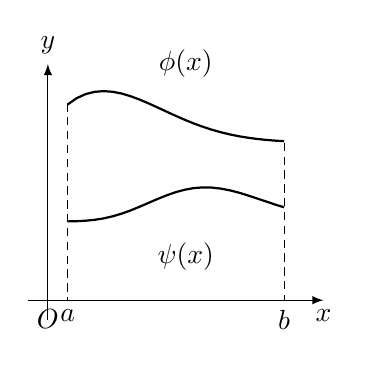
\begin{tikzpicture}[scale=1]
        \draw[-latex](-0.25,0) -- (3.5,0) node[below]{$x$};
        \draw[-latex](0,-0.25) -- (0,3) node[above]{$y$};
        \filldraw[black] (0,0) node[below]{$O$};
        \draw[black, thick, domain=0.25:3] plot (\x,{pow(\x,0.5)*pow(e,-\x*\x/2)+2});
        \filldraw[black] (1.75,3) node{$\phi(x)$};
        \draw[black, thick, domain=0.25:3] plot (\x,{pow(\x,4)*pow(e,-\x*\x/2)/5+1});
        \filldraw[black] (1.75,0.55) node{$\psi(x)$};
        \draw[black, densely dashed](0.25,2.5) -- (0.25,0) node[below]{$a$};
        \draw[black, densely dashed](3,2) -- (3,0) node[below]{$b$};
    \end{tikzpicture}
\end{minipage}

\paragraph{\texorpdfstring{$Y$}型区域} \leavevmode \medskip

\begin{minipage}{0.3\linewidth}
    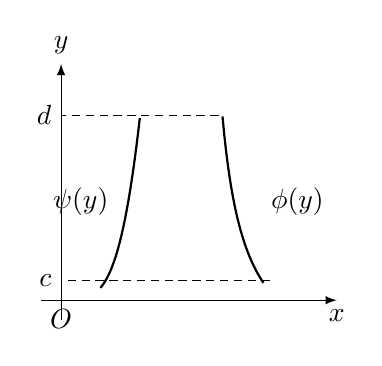
\begin{tikzpicture}[scale=1]
        \draw[-latex](-0.25,0) -- (3.5,0) node[below]{$x$};
        \draw[-latex](0,-0.25) -- (0,3) node[above]{$y$};
        \filldraw[black] (0,0) node[below]{$O$};
        \draw[black, thick, domain=2.05:2.57] plot (\x,{pow(\x-1.75,-1)-1});
        \filldraw[black] (3,1.25) node{$\phi(y)$};
        \draw[black, thick, domain=0.5:1] plot (\x,{pow(\x+0.25,6)*pow(e,-\x*\x/2)});
        \filldraw[black] (0.25,1.25) node{$\psi(y)$};
        \draw[black, densely dashed](2.65,0.25) -- (0,0.25) node[left]{$c$};
        \draw[black, densely dashed](2,2.35) -- (0,2.35) node[left]{$d$};
    \end{tikzpicture}
\end{minipage}
\hfill
\begin{minipage}{0.5\linewidth}
    也称为左右型区域。

    $\iint\limits_Df(x,y)\,\textrm{d}\sigma=\int_c^d\textrm{d}y\int_{\psi(y)}^{\phi(y)}f(x,y)\,\textrm{d}x$。
\end{minipage}

\paragraph{区域类型选择} \leavevmode \medskip

若上下是两条曲线,那么就是$X$型,若左右是两条曲线,那么就是$Y$型。

若同一个方向的函数有两种不同的表达式,则从另一个方向将$D$按照函数分段割开求积分。

\subsubsection{极坐标系}

按积分区域与极点位置关系的不同,将二重积分计算分为三种情况:

根据$\theta$按角度切割区间,然后从极点开始按$\textrm{d}r$切割,变成一个个类似矩形的图形。图形一边为切割半径的改变量$\textrm{d}r$,另一条边为圆弧,等于半径乘改变角度$r\textrm{d}\theta$,所以最后$\textrm{d}\sigma=r\textrm{d}r\textrm{d}\theta$。

基本上都是先积$r$后积$\theta$。

从射线刚开始接触区域$D$的射线记为$\theta=\alpha$,要离开区域$D$的射线记为$\theta=\beta$,中间移动的射线为$\theta=\theta$。$\theta=\alpha$与$\theta=\beta$与$D$相交于两点,两点内靠近极点的$D$的边为\textbf{内曲线},远离极点的边为\textbf{外曲线}。$\theta=\theta$与内曲线交于$r=r_1(\theta)$,与外曲线交于$r=r_2(\theta)$。

\begin{enumerate}
    \item 极点$O$在区域$D$外部:$\iint\limits_Df(x,y)\,\textrm{d}\sigma=\int_\alpha^\beta\textrm{d}\theta\int_{r_1(\theta)}^{r_2(\theta)}f(r\cos\theta,r\sin\theta)r\,\textrm{d}r$。
    \item 极点$O$在区域$D$边上:$\iint\limits_Df(x,y)\,\textrm{d}\sigma=\int_\alpha^\beta\textrm{d}\theta\int_0^{r(\theta)}f(r\cos\theta,r\sin\theta)r\,\textrm{d}r$。
    \item 极点$O$在区域$D$内部:$\iint\limits_Df(x,y)\,\textrm{d}\sigma=\int_0^{2\pi}\textrm{d}\theta\int_0^{r(\theta)}f(r\cos\theta,r\sin\theta)r\,\textrm{d}r$。
\end{enumerate}

\subsubsection{极坐标系与直角坐标系选择}

若给出一个二重积分:

\begin{enumerate}
    \item 被积函数是否为$f(x^2+y^2)$、$f\left(\dfrac{y}{x}\right)$、$f\left(\dfrac{x}{y}\right)$等形式。
    \item 积分区域是否为圆或圆的一部分。
    \item 如果上面两种都有,则优先使用极坐标系,否则优先考虑直角坐标系。
\end{enumerate}

\subsubsection{极直互化}

对于极坐标系转换到直角坐标系:$x=r\cos\theta$,$y=r\sin\theta$。

\textbf{例题:}设区域$D=\{(x,y)|x^2+y^2\leqslant R^2\}$,计算$\displaystyle{\iint\limits_D\left(\dfrac{x^2}{a^2}+\dfrac{y^2}{b^2}\right)\textrm{d}x\textrm{d}y}$。

解:互换积分变量:$I=\displaystyle{\iint\limits_D\left(\dfrac{x^2}{a^2}+\dfrac{y^2}{b^2}\right)\textrm{d}x\textrm{d}y}=\displaystyle{\iint\limits_D\left(\dfrac{y^2}{a^2}+\dfrac{x^2}{b^2}\right)\textrm{d}x\textrm{d}y}$。

$\therefore2I=\left(\dfrac{1}{a^2}+\dfrac{1}{b^2}\right)\displaystyle{\iint\limits_D(x^2+y^2)\textrm{d}x\textrm{d}y}$,$\therefore I=\dfrac{1}{2}\left(\dfrac{1}{a^2}+\dfrac{1}{b^2}\right)\displaystyle{\iint\limits_D(x^2+y^2)\textrm{d}\sigma}$。

根据公式三转换为极坐标系:$I=\dfrac{1}{2}\left(\dfrac{1}{a^2}+\dfrac{1}{b^2}\right)\int_0^{2\pi}\textrm{d}\theta\int)^Rr^2r\,\textrm{d}r$。

即$I=\left(\dfrac{1}{a^2}+\dfrac{1}{b^2}\right)\dfrac{\pi R^4}{4}$。

\textbf{例题:}计算$I=\int_0^1\textrm{d}x\int_{1-x}^{\sqrt{1-x^2}}\dfrac{x+y}{x^2+y^2}\textrm{d}y$。

解:根据上限$\sqrt{1-x^2}$和$1-x$所围成的图形$D$为第一象限的圆减去三角形。

所以转换为极坐标系时,对于$\theta\in\left(0,\dfrac{\pi}{2}\right)$,对于$r$在$(1-x,\sqrt{1-x^2})$。

下限$x+y=1$,即$r\cos\theta+r\sin\theta=1$,解出$r=\dfrac{1}{\cos\theta+\sin\theta}$,上限是一个圆,所以为1。

$=\int_0^\frac{\pi}{2}\textrm{d}\theta\int_\frac{1}{\cos\theta+\sin\theta}^1\cos\theta+\sin\theta\,\textrm{d}r=\int_0^\frac{\pi}{2}\cos\theta+\sin\theta-1\,\textrm{d}\theta=2-\dfrac{\pi}{2}$。

\subsubsection{积分次序}

积分次序即区域类型选择的问题,目的是为了简化计算,使得积分的函数更简单。

从另一方面,也很可能是积分函数无法按此次序进行积分,所以需要更换积分顺序。

存在许多有原函数但求不出初等函数形式的原函数。如$\dfrac{\sin x}{x}$、$\dfrac{\cos x}{x}$、$\dfrac{\tan x}{x}$、$\dfrac{e^x}{x}$、$\sin x^2$、$\cos x^2$、$\tan x^2$、$e^{ax^2+bx+c}$、$\dfrac{1}{\ln x}$等。

\textbf{例题:}计算$\displaystyle{\int_1^2\textrm{d}x\int_{\sqrt{x}}^x\sin\dfrac{\pi x}{2y}\textrm{d}y+\int_2^4\textrm{d}x\int_{\sqrt{x}}^2\sin\dfrac{\pi x}{2y}\textrm{d}y}$。

解:首先可以看出积分函数都是一样的,只是积分区域不同所以分开了,可见该函数的积分区域较复杂。

积分函数为$\sin\dfrac{\pi x}{2y}$,若对$y$进行积分,则可以类比求$\displaystyle{\int\sin\dfrac{1}{x}\,\textrm{d}x}$,这个是积分积不出来的。所以必须更换积分顺序。先积$x$。

首先根据被积函数上下限得到积分区域:$\sqrt{x}$、$x$、2围成的类三角形$\textrm{d}\sigma$。

$I=\displaystyle{\iint\limits_D\sin\dfrac{\pi x}{2y}\textrm{d}\sigma}=\displaystyle{\int_1^2\textrm{d}y\int_y^{y^2}\sin\dfrac{\pi x}{2y}\textrm{d}x}=\displaystyle{\int_1^2\dfrac{2y}{\pi}\left(-\cos\dfrac{\pi y}{2}+\cos\dfrac{\pi}{2}\right)}\textrm{d}y=\dfrac{4}{\pi^3}(2+\pi)$。

\subsubsection{二重积分处理一元积分}

在面对有中间变量的一元积分时,可以使用二重积分。

\textbf{例题:}设$f(x)=\int_x^1\sin(\pi u^2)\,\textrm{d}u$,求$\int_0^1f(x)\,\textrm{d}x$。(可以使用分部积分法)

解:$\int_0^1f(x)\,\textrm{d}x=\int_0^1\textrm{d}x\int_x^1\sin(\pi u^2)\,\textrm{d}u$。又$\sin(\pi u^2)$无法对$x$积分。

换做对$y$积分,$\textrm{d}\sigma$为$x=0$、$x=1$、$u=x$围成的三角形。交换积分次序:

$\int_0^1\textrm{d}y\int_0^u\sin(\pi u^2)\,\textrm{d}x=\int_0^1\sin(\pi u^2)u\,\textrm{d}u=\dfrac{1}{2\pi}\int_0^1\sin(\pi u^2)\,\textrm{d}(\pi u^2)=-\dfrac{1}{2\pi}$\\$\cos\pi u^2|_0^1=-\dfrac{1}{2\pi}(-1-1)=\dfrac{1}{\pi}$。

\textbf{例题:}利用广义二重积分求$\int_0^{+\infty}e^{-x^2}\,\textrm{d}x$。

解:根据积分值与积分变量无关的性质:

$I^2=(\int_0^{+\infty}e^{-x^2}\,\textrm{d}x)^2=\int_0^{+\infty}e^{-x^2}\,\textrm{d}x\cdot\int_0^{+\infty}e^{-y^2}\,\textrm{d}y=\int_0^{+\infty}\int_0^{+\infty}e^{-x^2-y^2}\,\textrm{d}x\textrm{d}y$。

$\textrm{d}\sigma$是第一象限,可以看作一个广义的圆,半径无限大,转换为极坐标系。

$=\int_0^\frac{\pi}{2}\textrm{d}\theta\int_0^{+\infty}e^{-r^2}r\,\textrm{d}r=\displaystyle{\int_0^\frac{\pi}{2}\dfrac{1}{2}\,\textrm{d}\theta}=\dfrac{\pi}{2}$。$\therefore I=\dfrac{\sqrt{\pi}}{2}$。

\section{三重积分}

\section{曲线曲面积分}

\end{document}
